\documentclass[11pt]{article}
\usepackage{graphicx}  % Include figure files
\usepackage{amsmath}

\begin{document}

%
%Such a stability
\section*{Addendum to Reply from Tuesday, Aug. 11, 2020}

\subsection*{Impact of efficiency ratio on the neutron / proton yields ratio}

{\hskip 0.7cm}We want to evaluate the impact of the ratio of hadron efficiencies,\\
$R_{\eta_{n/p}} = \eta_n/\eta_p$
on the ratio of neutrons to proton yields $R_{n/p} = N_{en}/N_{ep}$.

To obtain the ``true'' ratio of neutrons to proton yields $R_{n/p}$ from the recorded ``raw''
ratio of neutrons to proton yields $R_{n/p, raw}$,
this ratio needs to be corrected by $R_{n/p}$.
%
\begin{equation}
  R_{n/p} = R_{n/p, raw}/R_{\eta_{n/p}}
\end{equation}
%
Hence, the uncertainty, $\Delta R_{n/p}$ of $R_{n/p}$ could be expressed as:
%
\begin{equation}
  \Delta R_{n/p}/R_{n/p} = \Delta R_{\eta_{n/p}}/R_{\eta_{n/p}}.
\end{equation}
%
To evaluate the uncertainty of $R_{\eta_{n/p}} = \eta_p/\eta_n$,
we need to account for the strong correlation between $\eta_p$ and $\eta_n$, $\rho_{\eta_{n/p}}$. 
We can define the covariance between the uncertainties $\Delta \eta_p$ and $\Delta \eta_n$,
$\sigma_{\eta_{n/p}} = \rho_{\eta_{n/p}} \Delta \eta_{n} \Delta \eta_{p}$ \footnote{https://en.wikipedia.org/wiki/Covariance\_and\_correlation}.

According to\footnote{https://www.sagepub.com/upm-data/6427\_Chapter\_4\_\_Lee\_(Analyzing)\_I\_PDF\_6.pdf}, we can write the uncertainty on the ratio efficiencies:
%\footnote{line~5 of table in https://en.wikipedia.org/wiki/Propagation\_of\_uncertainty\#Example\_formulae}

%
%\begin{equation}
\begin{align}
  \frac{\Delta R_{\eta_{n/p}}}{R_{\eta_{n/p}}} &= \sqrt{ \left( \frac{\Delta \eta_{n}}{\eta_{n}} \right)^2
    + \left( \frac{\Delta \eta_{p}}{\eta_{p}} \right)^2
    - 2 \frac{\sigma_{\eta_{n/p}}}{\eta_{n}\eta_{p}} }
  \\
  &= \sqrt{ \left( \frac{\Delta \eta_{n}}{\eta_{n}} \right)^2
    + \left( \frac{\Delta \eta_{p}}{\eta_{p}} \right)^2
    - 2 \frac{\rho_{\eta_{n/p}} \Delta\eta_{n} \Delta\eta_{p}}{\eta_{n}\eta_{p}} }
  \label{eq:uncert_exact}
  %\end{equation}
\end{align}
%
\begin{figure}[!h]
  \centering
  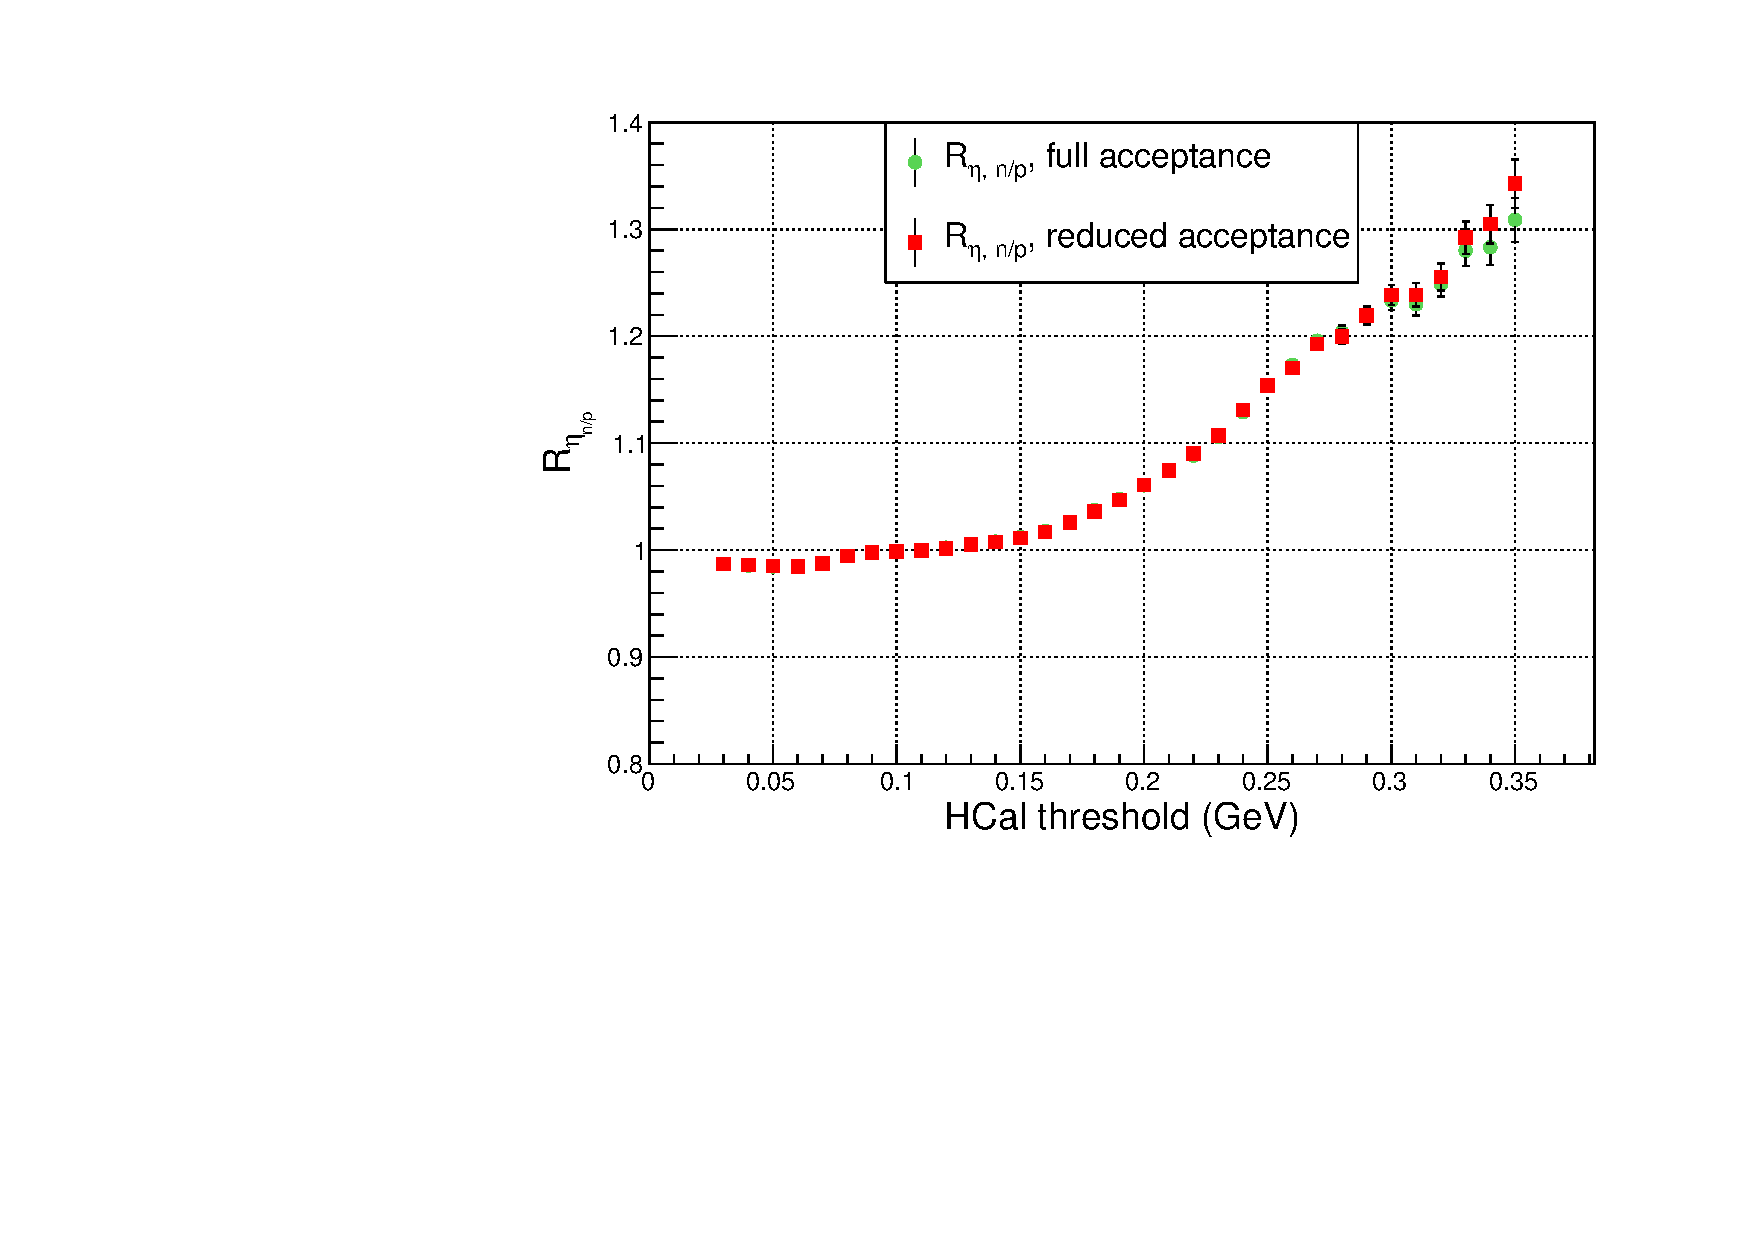
\includegraphics[width=7cm]{Reta_np_fthr_errs.pdf}
  \caption{Neutron/proton efficiency ratio $R_{\eta_{n/p}}$ as a function of the calorimeter threshold, for our quasi-elastic sample. The error bars represent the uncertainty from the calibration measurements discussed earlier. The green represents $R_{\eta_{n/p}}$ on the full acceptance, the red represents $R_{\eta_{n/p}}$ on a reduced acceptance.
    % The discrepancy between the two (blue) is about 0.1\% below a threshold of 0.15 GeV.%, but becomes about 0.5\% between 0.15 and 0.3 GeV, up to 1\% beyond 0.3 GeV}
  }
  \label{fig:Reta_np}
\end{figure}
%
$\Delta\eta_{p}$ and $\Delta\eta_{n}$ are the uncertainties from the calibration measurements described on the Monday write up. %$\sigma_{\eta-n/p}$. Fig~\ref{fig:Reta_np}.
The correlation between the variations of the proton and neutron efficiencies $\rho_{\eta_{n/p}}$, depends on the cause of the variations.
In the case of the efficiency calibrations runs, discussed in the Monday write-up,
the uncertainties of the efficiencies are due to the statistic of the collected events. 
In such a case, $\rho_{\eta_{n/p}} = 0$.
However, in the case of the detector instability, $\rho_{\eta_{n/p}} \sim 1$ (see again Fig.~\ref{fig:Reta_np}).

With the statistics projected for the calibration runs: $\eta_p \pm \Delta\eta_{p} = 0.915 \pm 0.003$ and $\eta_n \pm \Delta\eta_{n} = 0.924 \pm 0.014$.
Applying these values to Eq.~\ref{eq:uncert_exact}, %, and considering $R_{\eta_{n/p}} = 0.991$,
the relative uncertainty on the absolute value of the hadron efficiency ratio becomes:
%
\begin{equation}
  \Delta R_{\eta_{n/p}}/R_{\eta_{n/p}} = 1.6\%.
\end{equation}
%
Considering $R_{\eta_{n/p}} = 0.991$ from Fig.~\ref{fig:Reta_np}, $\Delta R_{n/p}/R_{n/p} = 0.016$. 
This would add up to the total systematic uncertainty of $R_{n/p}$ to 1.9\% for the low $\epsilon$ kinematic and to 1.6\% for the high $\epsilon$ kinematic.\\

However, %as it was demonstrated in Tuesday's write-up,
the measurement of the Rosenbluth slope, $S^n = \sigma_L/\sigma_T$, is unaffected by the uncertainty of the absolute value of the efficiency ratio $R_{\eta_{n/p}}$.
$R_{\eta_{n/p}}$ will be cancelled in the the determination of the neutron Rosenbluth slope $S^n$, 
{\it as long as we control the stability of $R_{\eta_{n/p}}$ over the few days of the measurement}.
%
\newpage

\subsection*{Efficiency stability due to the detector parameters drift}

As we know, the stability of the hadron detector efficiency is critical for a successful measurement.
The instability of the efficiency $\eta$ over time is mainly due to the drift of the PMTs signals and the related electronics.
Such an amplitude drift is typically of 1-2\% over a few days.
It will be better for our detector thanks to the LED calibration system.

We expect to use a threshold $A_{thr}$ = 100 MeV (see plots of amplitude spectrum in the Monday write-up).
Using the graph of the nucleon detection efficiency as a function of the threshold $A_{thr}$ on Fig.~\ref{fig:eta_N},
we find that, in the region $A_{thr} = 90 - 110$~MeV, the efficiency is:
%
\begin{equation}
  \eta = 0.92 - 0.18 \times \frac{A[{\rm MeV}]-100}{100}
\end{equation}
%
A one percent variation of $A_{thr}$ leads to 0.2\% variation of efficiency.
%
\begin{figure}[!h]
  \centering
  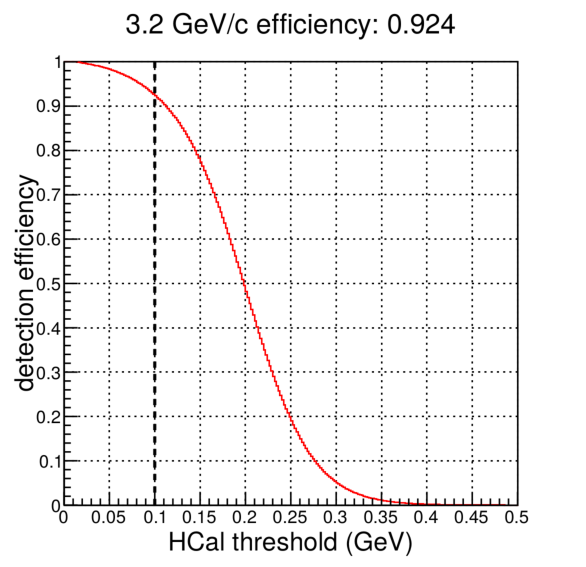
\includegraphics[width=7cm]{Neff_fThr.pdf}
  \caption{Nucleon detection efficiency vs the calorimeter threshold $A_{thr}$.}
  \label{fig:eta_N}
\end{figure}
%

Turning now to the ratio of efficiencies, we plot it as a function of the threshold on Fig.~\ref{fig:Reta_np}.
We find that, in the region $A_{thr} = 90 - 110$~MeV, the ratio of efficiencies is:
%
\begin{equation}
  R_{\eta_{n/p}} = \frac{\eta_n}{\eta_p} = 0.998 + 0.011 \times \frac{A[{\rm MeV}]-100}{100}.
\end{equation}
%
Using the estimate for a PMT-based system instability of 1-2\%, which means that $A_{thr}$ is stable to 1-2 MeV,
the ratio of efficiencies $R_{\eta_{n/p}} = \frac{\eta_n}{\eta_p}$ is found to be stable to 0.022\%.

The run plan of the GMn experiment (E12-09-019), which will run next summer,
has a provision of running on the hydrogen target multiple times with different fields in the SBS dipole,
allowing the study of the stability of individual modules of HCal.


\end{document}
